%===============================================================================
\section{Unidades de medida y forma funcional}
%===============================================================================
\begin{frame}{Formas funcionales}
	\begin{figure}
		\centering
		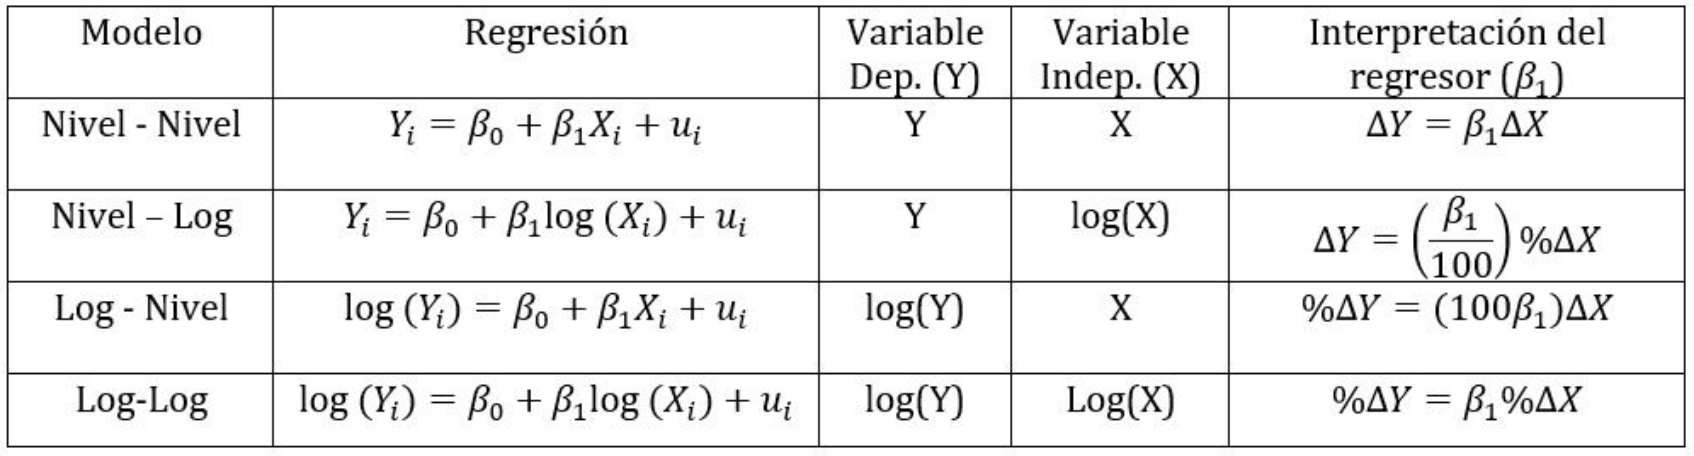
\includegraphics[width=0.9\linewidth]{fig/form_fun.png}
	\end{figure}
	\begin{itemize}
		\item El modelo Nivel-Nivel representa las variables en su forma original (regresión en forma lineal). Es decir, un cambio de una unidad en $X$, afecta en $\beta_1$ unidades a $Y$.
		\item El modelo Nivel-Log se interpreta como un incremento del 1\% de cambio en $X$ es asociado a un cambio en $Y$ de 0,01$\cdot\beta_1$.
		\item El modelo Log-Nivel es el menor frecuentemente utilizado y se conoce como la semielasticidad de $Y$ respecto a $X$. Se interpreta como un incremento de 1 unidad en $X$ es asociado a un cambio en Y de (100$\cdot\beta_1$ )\%.
		\item El modelo Log-Log es atribuye a $\beta_1$ la elasticidad de $Y$, respecto a $X$. Se interpreta como un incremento del 1\% en $X$ es asociado a un cambio en $Y$ de $\beta_1$\%.
	\end{itemize}
\end{frame}